\documentclass[A4paper, 11pt]{article}

%\usepackage[UTF8]{ctex}
\usepackage{amsfonts}
\usepackage{amsmath} 
\usepackage{amssymb}
\usepackage{array}
\usepackage{booktabs}
\usepackage{bm}
\usepackage{cite}
\usepackage{colortbl}
\usepackage{enumerate}
\usepackage{extarrows}
\usepackage{float}
\usepackage{geometry}
\usepackage{graphics}
\usepackage{graphicx}
\usepackage{ifthen}
\usepackage{listings}
\usepackage{longtable}
\usepackage{multicol}
\usepackage{pgf}
\usepackage{pgfplots}
\usepackage{pifont}
\usepackage{pstricks}
\usepackage{pst-node}
\usepackage{pst-tree}
\usepackage{pythonhighlight}
\usepackage{setspace}
\usepackage{tabularx}
\usepackage{tikz}
\usepackage{tocloft}
\usepackage{wrapfig}

\geometry{left=2cm, right=2cm, top=2cm, bottom=2cm}

\definecolor{emph}{RGB}{0,100,141}

\newcommand{\tabincell}[2]{\begin{tabular}{@{}#1@{}}#2\end{tabular}}
\newcommand*{\circled}[1]{\lower.7ex\hbox{\tikz\draw (0pt, 0pt) circle (.5em) node {\makebox[1em][c]{\small #1}};}}
\newcommand{\sfrac}[2]{\mbox{\small$\dfrac{#1}{#2}$}}
\renewcommand{\geq}{\geqslant}
\renewcommand{\leq}{\leqslant}
\renewcommand{\vec}{\overrightarrow}
\renewcommand{\d}{\,\mathrm{d}}
\newcommand{\lto}{\longrightarrow}
\newcommand{\ex}{\exists\,}
\newcommand{\R}{\mathbb{R}}
\newcommand{\<}{\,\langle\,}
\renewcommand{\>}{\,\rangle}
\newcommand{\normuv}[1]{\big|{#1}(u,v)\big|^2}
\newcommand{\infint}{\int_{-\infty}^{+\infty}}
\newcommand{\hollowstar}{\text{\ding{73}}}
\newcommand{\fullstar}{\text{\ding{72}}}

\newcommand{\Pro}[1]{\textbf{\large{Problem #1}} \vspace*{1ex}}
\newcommand{\Sol}{\textbf{\textit{Sol.}}}
\newcommand{\Ckp}{\textbf{\textit{Checkpoints}}}
\newcommand{\Pt}[1]{\textcolor{emph}{(#1 \ifthenelse{\equal{#1}{1}}{point}{points})}}

% Scalars
\renewcommand{\a}{\alpha}
% Matrices
\newcommand{\A}{\bm{A}}
\newcommand{\B}{\bm{B}}
\newcommand{\C}{\bm{C}}
\newcommand{\E}{\bm{E}}
% Vectors
\renewcommand{\b}{\bm{b}}
\newcommand{\x}{\bm{x}}
\newcommand{\y}{\bm{y}}
\newcommand{\z}{\bm{z}}
\renewcommand{\u}{\bm{u}}
\renewcommand{\v}{\bm{v}}
\newcommand{\w}{\bm{w}}
\newcommand{\0}{\mathbf{0}}
\newcommand{\1}{\mathbf{1}}
% Spaces
\newcommand{\V}{\mathcal{V}}
\newcommand{\X}{\mathcal{X}}
\newcommand{\Y}{\mathcal{Y}}
\newcommand{\F}{\mathcal{F}}
\newcommand{\N}{\mathcal{N}}
\renewcommand{\S}{\mathcal{S}}
% Names
\renewcommand{\sp}{\text{span}}
\newcommand{\rank}{\text{rank}}
\newcommand{\range}{\mathcal{R}}
\newcommand{\tr}{\text{tr}}

\newcommand{\typeset}{
    \setlength{\parindent}{0pt}
    \setlength{\parskip}{1ex}
    \setlength{\abovedisplayskip}{1ex}
    \setlength{\belowdisplayskip}{1ex}
}

\newcommand{\headbox}{
    \renewcommand{\arraystretch}{1.33}
    \begin{tabular}{|l|l|}
    \hline
    Name       & \hspace*{9em} \\
    \hline
    Student ID & \hspace*{9em} \\
    \hline
    \end{tabular} \hspace{131pt}
    \begin{tabular}{r}
        \textsc{CS\,270:\;Digital\;Image\;Processing} \\
        \textbf{\Large{Quiz 1}} \\
    \end{tabular}
    
    \vspace*{6ex}
    \renewcommand{\arraystretch}{1}
}

\begin{document}

\begin{spacing}{1.3}

\typeset

\textsc{\large{School\;of\;Information\;Science\;and\;Technology\\[2pt] ShanghaiTech\;University}}

\vspace*{5ex}

\textsc{\large{CS\,270:\;Digital\;Image\;Processing (Spring\;2024)}}

\vspace*{2.5ex} \textbf{\huge{Assignment 3}}

\vspace*{1.5ex} \textbf{\large{Due: 23:59, May 20, 2024}}

\vspace*{1.5ex} \textbf{\large{Name: Ruyue Yan, ID: 2020531005}}

\vspace*{5ex}

\textbf{\large{Notes}}

\begin{itemize} \setlength{\parskip}{0.5ex} \vspace*{-1ex} 
    \item This assignment has \textbf{100 points} in total.
    \item Please prepare all your solutions in English.
    \item Please prepare your report with digital typesetting software (LaTeX, Microsoft Word, etc.). Handwritten reports, including digital handwriting on iPad etc., will not be accepted.
    \item Please submit your assignment to \textbf{Blackboard} as a \textbf{zip} file with its name formatted as\\ \texttt{DIP2024\_HW3\_ID\_ChineseName.zip}. The zip file should contain 3 things:
    \begin{enumerate}
        \item Your report named as \texttt{HW3\_Report\_ID\_Name.pdf};
        \item A folder named as \texttt{code} that stores your codes;
        \item A folder named as \texttt{images} that stores the original images in your report.
    \end{enumerate}
    For each problem, you should provide a separate code file that corresponds to it, with its name like \texttt{p3.m} (for Problem 3) or \texttt{p6a.m} (for Problem 6 (a)). Please make sure all paths in your codes are relative paths, so that we can run your codes and get your results without any modification.
\end{itemize}

\vspace*{2ex}
\textbf{\large{Policy on Plagiarism}}
\vspace*{1.5ex}

This is an individual homework. You can discuss the ideas and algorithms, but:
\begin{itemize} \setlength{\parskip}{0.5ex} \vspace*{-1.5ex}
    \item You cannot read, modify, and submit the codes of other students, nor allow other students to read, modify, and submit your codes.
    \item You cannot directly use generative AI tools to produce codes for submission. While you may consult generative AI for understanding the ideas and algorithms, the code you submit must be the result of your own individual understanding and efforts.
\end{itemize} \vspace*{-1.5ex}
We will utilize automated tools to check for plagiarism, and any violations will result in a zero score for this assignment and $20\%$ discount on total course grade.

\newpage

\begin{center}
    \textsc{I. Coding Part}
\end{center}

Please complete all the coding assignments using MATLAB or python. Make sure your results in the report are the same as the results of your codes. For general operations, the following functions may be useful:\\
\texttt{load}, \texttt{imread}, \texttt{double}, \texttt{im2double}, \texttt{uint8}, \texttt{imshow}, \texttt{zeros}, \texttt{size}, \texttt{montage}, \texttt{subplot}, \texttt{bar}.

\textcolor{red}{You must implement the core code in each question WITHOUT using relevant build-in functions.}\\


\vspace*{-3.75ex}
You can type \texttt{\textbf{help} FunctionName} in Command Window of MATLAB for detailed help text for the functionality specified by \texttt{FunctionName}.

\vspace*{6ex}

\Pro{1: CT reconstruction}

In this task, we aim to perform a basic Computed Tomography (CT) image reconstruction using the Filtered Back Projection (FBP) algorithm. We will utilize the sinogram data provided in the file \texttt{sinogram.mat}, which contains projections from 180 angles. Our reconstruction will employ a Hamming-windowed Ramp filter for better image quality. \Pt{35}

\begin{figure}[h]
        \centering
        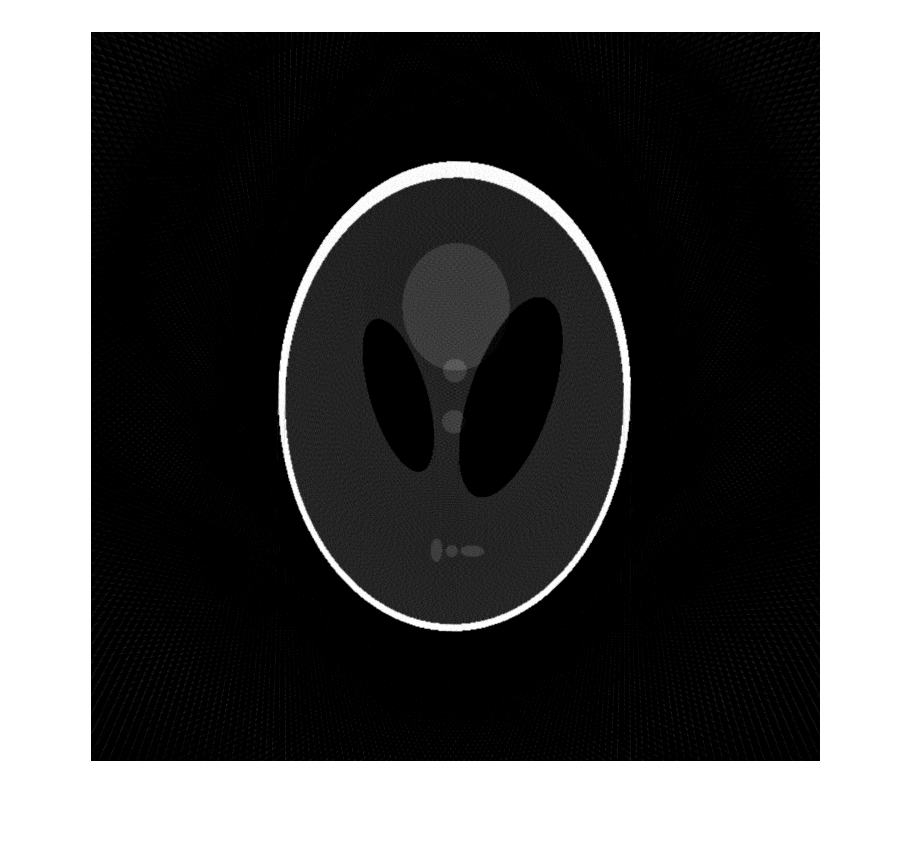
\includegraphics[width=0.5\textwidth]{./images/p1.png}
\end{figure}

\newpage
\Pro{2: Threshold processing}
\newline
(a) Please implement the Basic global thresholding on \texttt{flower.tif}. (start with T = 0.1). \Pt{15}

\begin{figure}[h]
	\centering
	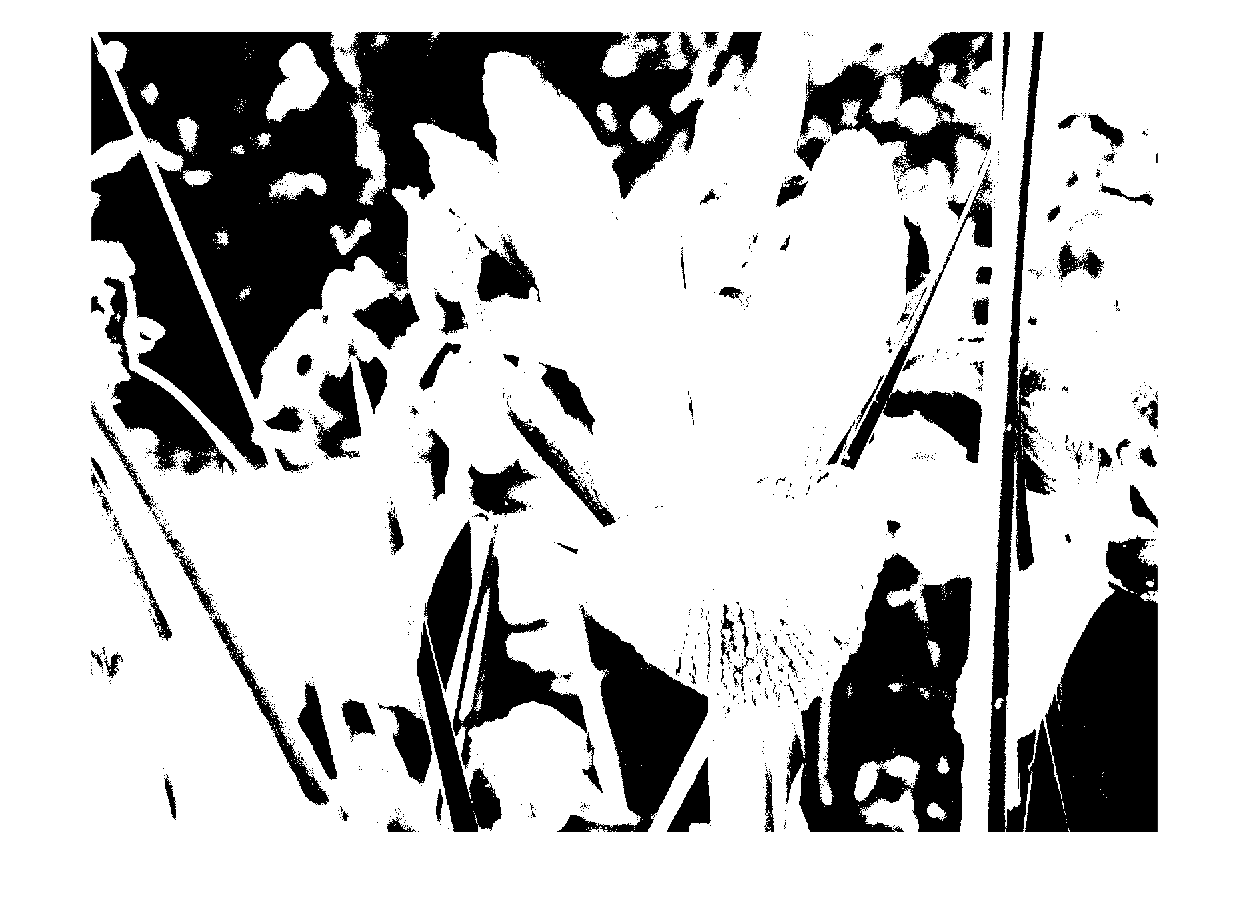
\includegraphics[width=0.5\textwidth]{./images/p2a.png}
\end{figure}

(b) Please implement the Region Splitting and Merging method on \texttt{nebula.jpg} to show the results of the minimum four-quadrant region size limit of 8*8 and 4*4 respectively. \Pt{15}
\newline
(Hint: Region Splitting and Merging based on the characteristics of mean and standard deviation of gray level of pixels in an area. Since the background standard deviation of the image is close to 0, and the average gray level of the nebula is greater than the mean gray level of the dark background, we believe that:
\[
Q =
\begin{cases}
    TRUE, &  \sigma > a \text{ and } 0 < m < b \\
    FALSE,  & otherwise
\end{cases}
\]
For this task, the value of $a$ is set to 0.7, and the value of $b$ is set to 170. For the result image, the area pixels that satisfy the attribute are set to white, and the other pixels are set to black.)

\begin{figure}[h]
	\centering
	\begin{minipage}{0.48\textwidth}
		\centering
		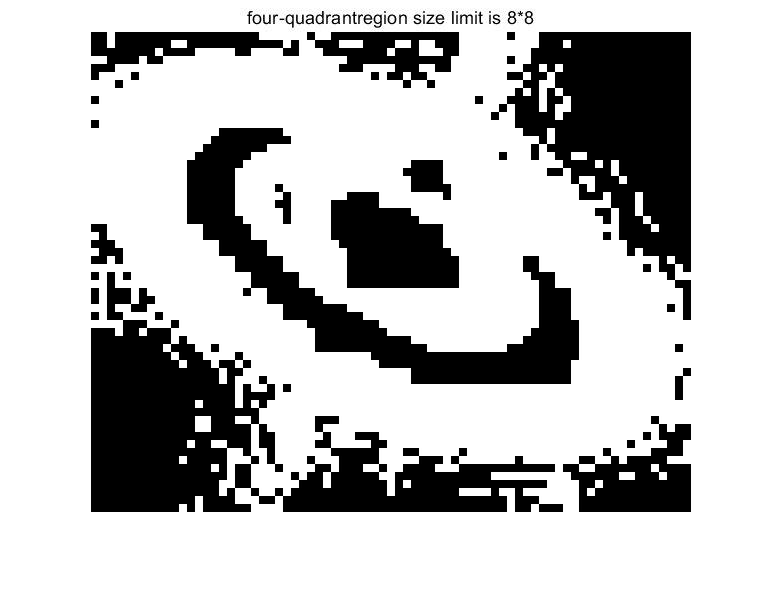
\includegraphics[width=0.9\textwidth]{./images/p2b_8.png}
		\caption{four-quadrant size limit 8*8}
	\end{minipage}
	\begin{minipage}{0.48\textwidth}
		\centering
		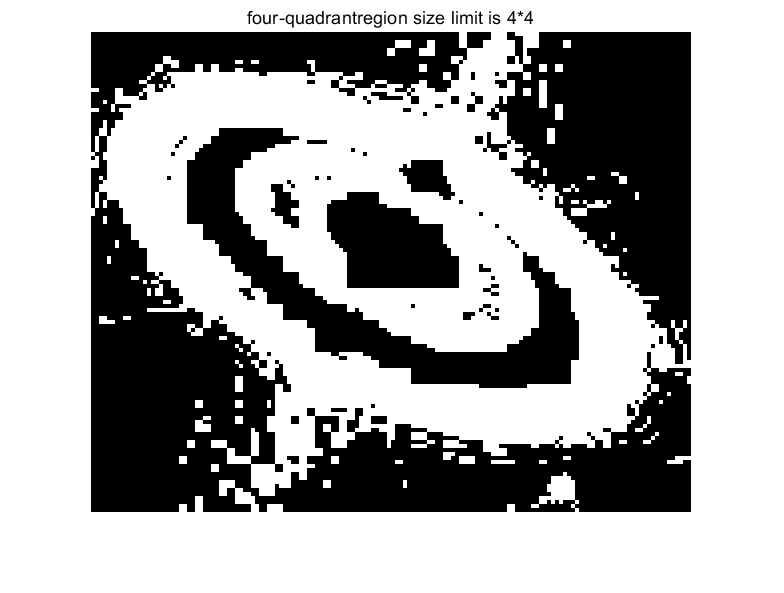
\includegraphics[width=0.9\textwidth]{./images/p2b_4.png}
		\caption{four-quadrant size limit 4*4}
	\end{minipage}
\end{figure}

\newpage
\Pro{3: Super pixel}

Super pixel is a method that turns a pixel-level picture into district-level pictures, which is an abstraction of basic information elements. A super pixel is a small area composed of a series of adjacent pixels with similar characteristics such as color, brightness, and texture. Most of these small areas retain effective information for further image segmentation, and generally do not destroy the boundary information of objects in the image.

In this problem, you need to turn \texttt{seahouse.jpg} to super pixel style using SLIC algorithm with cluster center 100, 500 and 1000 (In practice, number of cluster center can be different with these values, but should be close to these values) show the result images. \Pt{35}

Reference, doi: 10.1109/TPAMI.2012.120. \\

\hspace*{\fill}\\
compactness = 10
\begin{figure}[h]
	\centering
	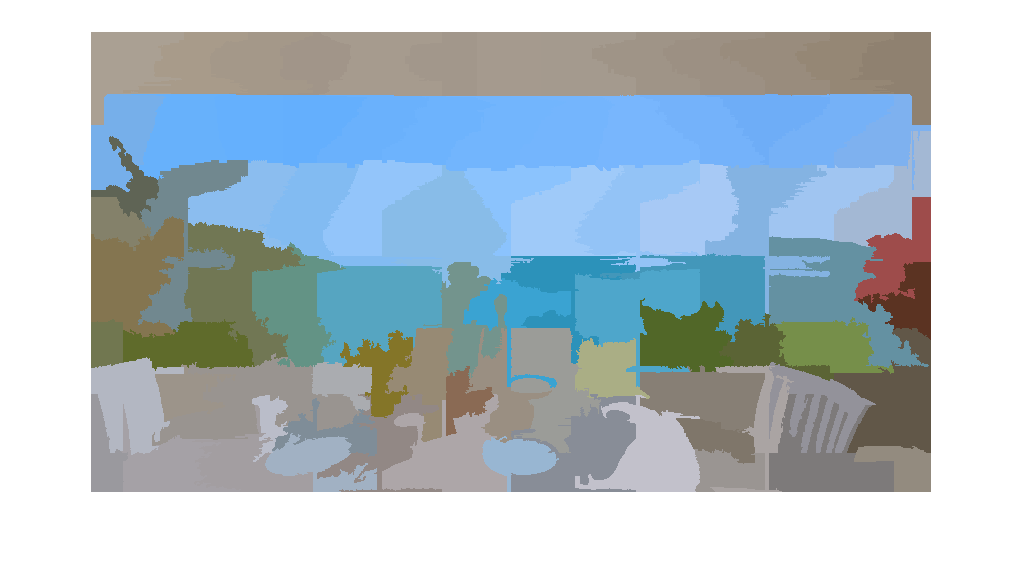
\includegraphics[width=0.8\textwidth]{./images/p3_100.png}
	\caption{number of cluster number is 100}
\end{figure}
\begin{figure}[h]
	\centering
	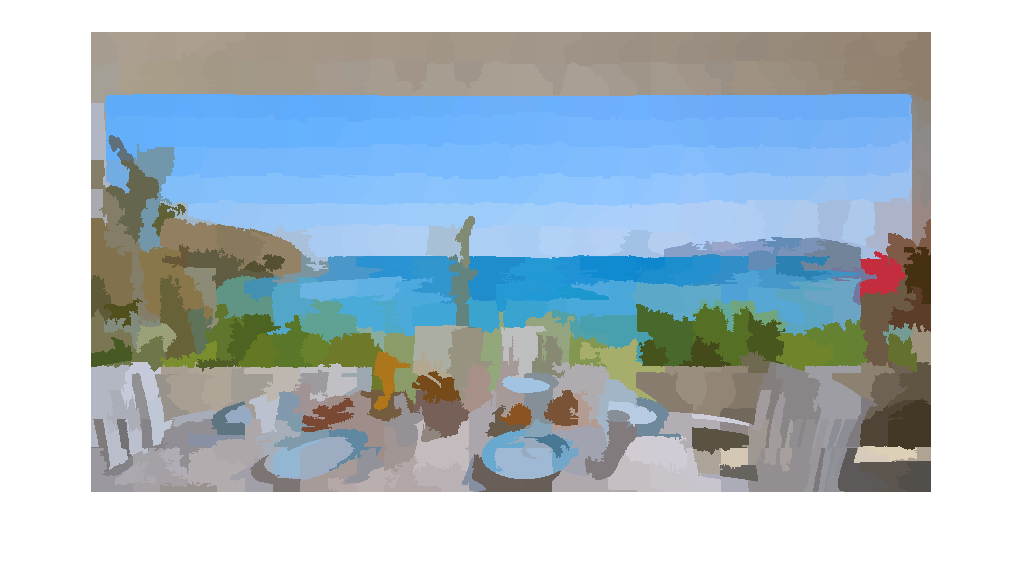
\includegraphics[width=0.8\textwidth]{./images/p3_500.png}
	\caption{number of cluster number is 500}
\end{figure}
\begin{figure}[h]
	\centering
	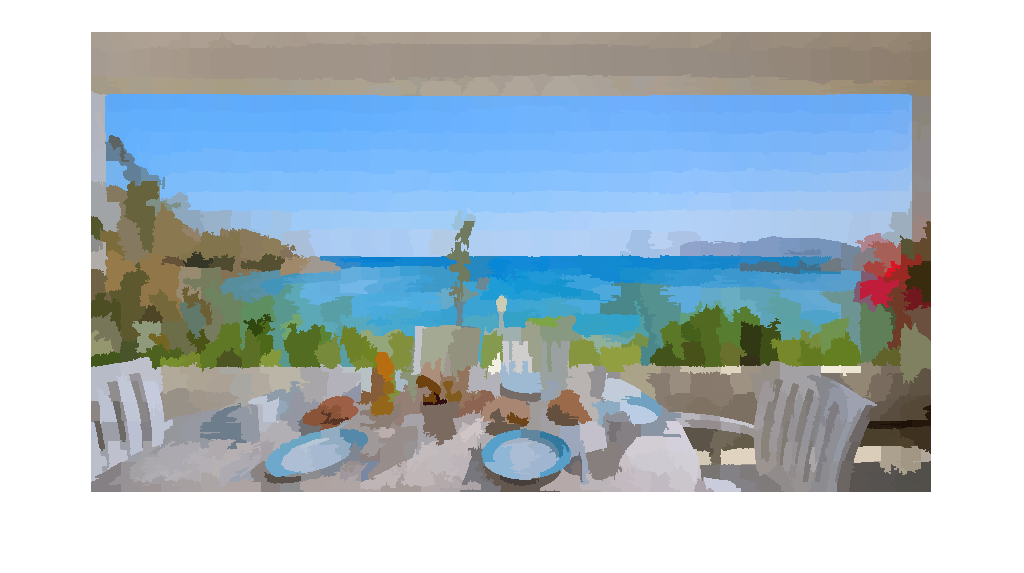
\includegraphics[width=0.8\textwidth]{./images/p3_1000.png}
	\caption{number of cluster number is 1000}
\end{figure}

\newpage


\end{spacing}



\end{document}